
\subsection{Caractéristiques générales de la carte acoustique}

\subsubsection{Caractéristiques physiques de la carte acoustique}
Les caractéristiques physiques de la carte acoustique respectent les standards suivants:\\

\begin{itemize}
\item \textbf{ISO 7810:} la carte a été certifiée conforme. Ce format est celui de la carte bancaire (85.60 x 53.98 mm)
\item \textbf{ISO 7811:} ce standard est une extension de l’ISO 7810. Il décrit les techniques d’enregistrement d’identité sur la carte: embossage et piste magnétique.
\item \textbf{ISO 7816:} la carte est compatible avec cet ISO si l’on souhaite y apposer une puce de type EMV
\item \textbf{ISO 14443:} la carte peut être équipée d’une puce et d’une antenne RFID (13.56 MHz)
\end{itemize}

\begin{figure}[!htbp]
  \centering
    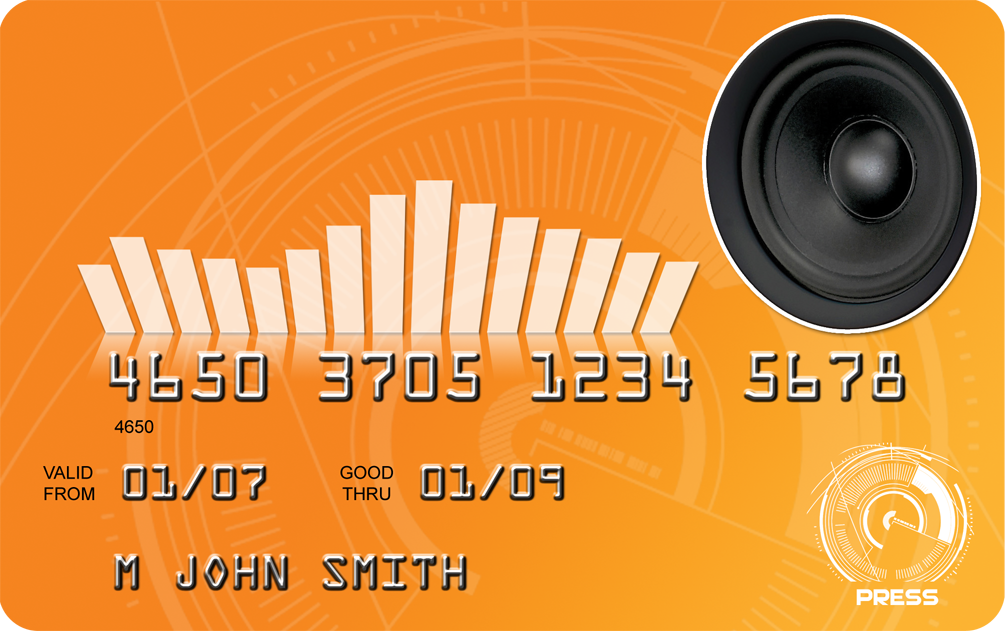
\includegraphics[scale=0.5]{images/carteavant}
  \caption{Face avant d’une carte acoustique}
  %\label{fig:auth}
\end{figure}


\subsubsection{Fonctionnalités générales}

La carte acoustique émet une séquence acoustique unique à chaque pression du bouton.
La carte utilise un microprocesseur pour calculer les deux OTP (One Time Password).
L’énergie utilisée provient d’une batterie fine et flexible.

\subsubsection{Schéma d’une carte acoustique}
\begin{figure}[!htbp]
  \centering
    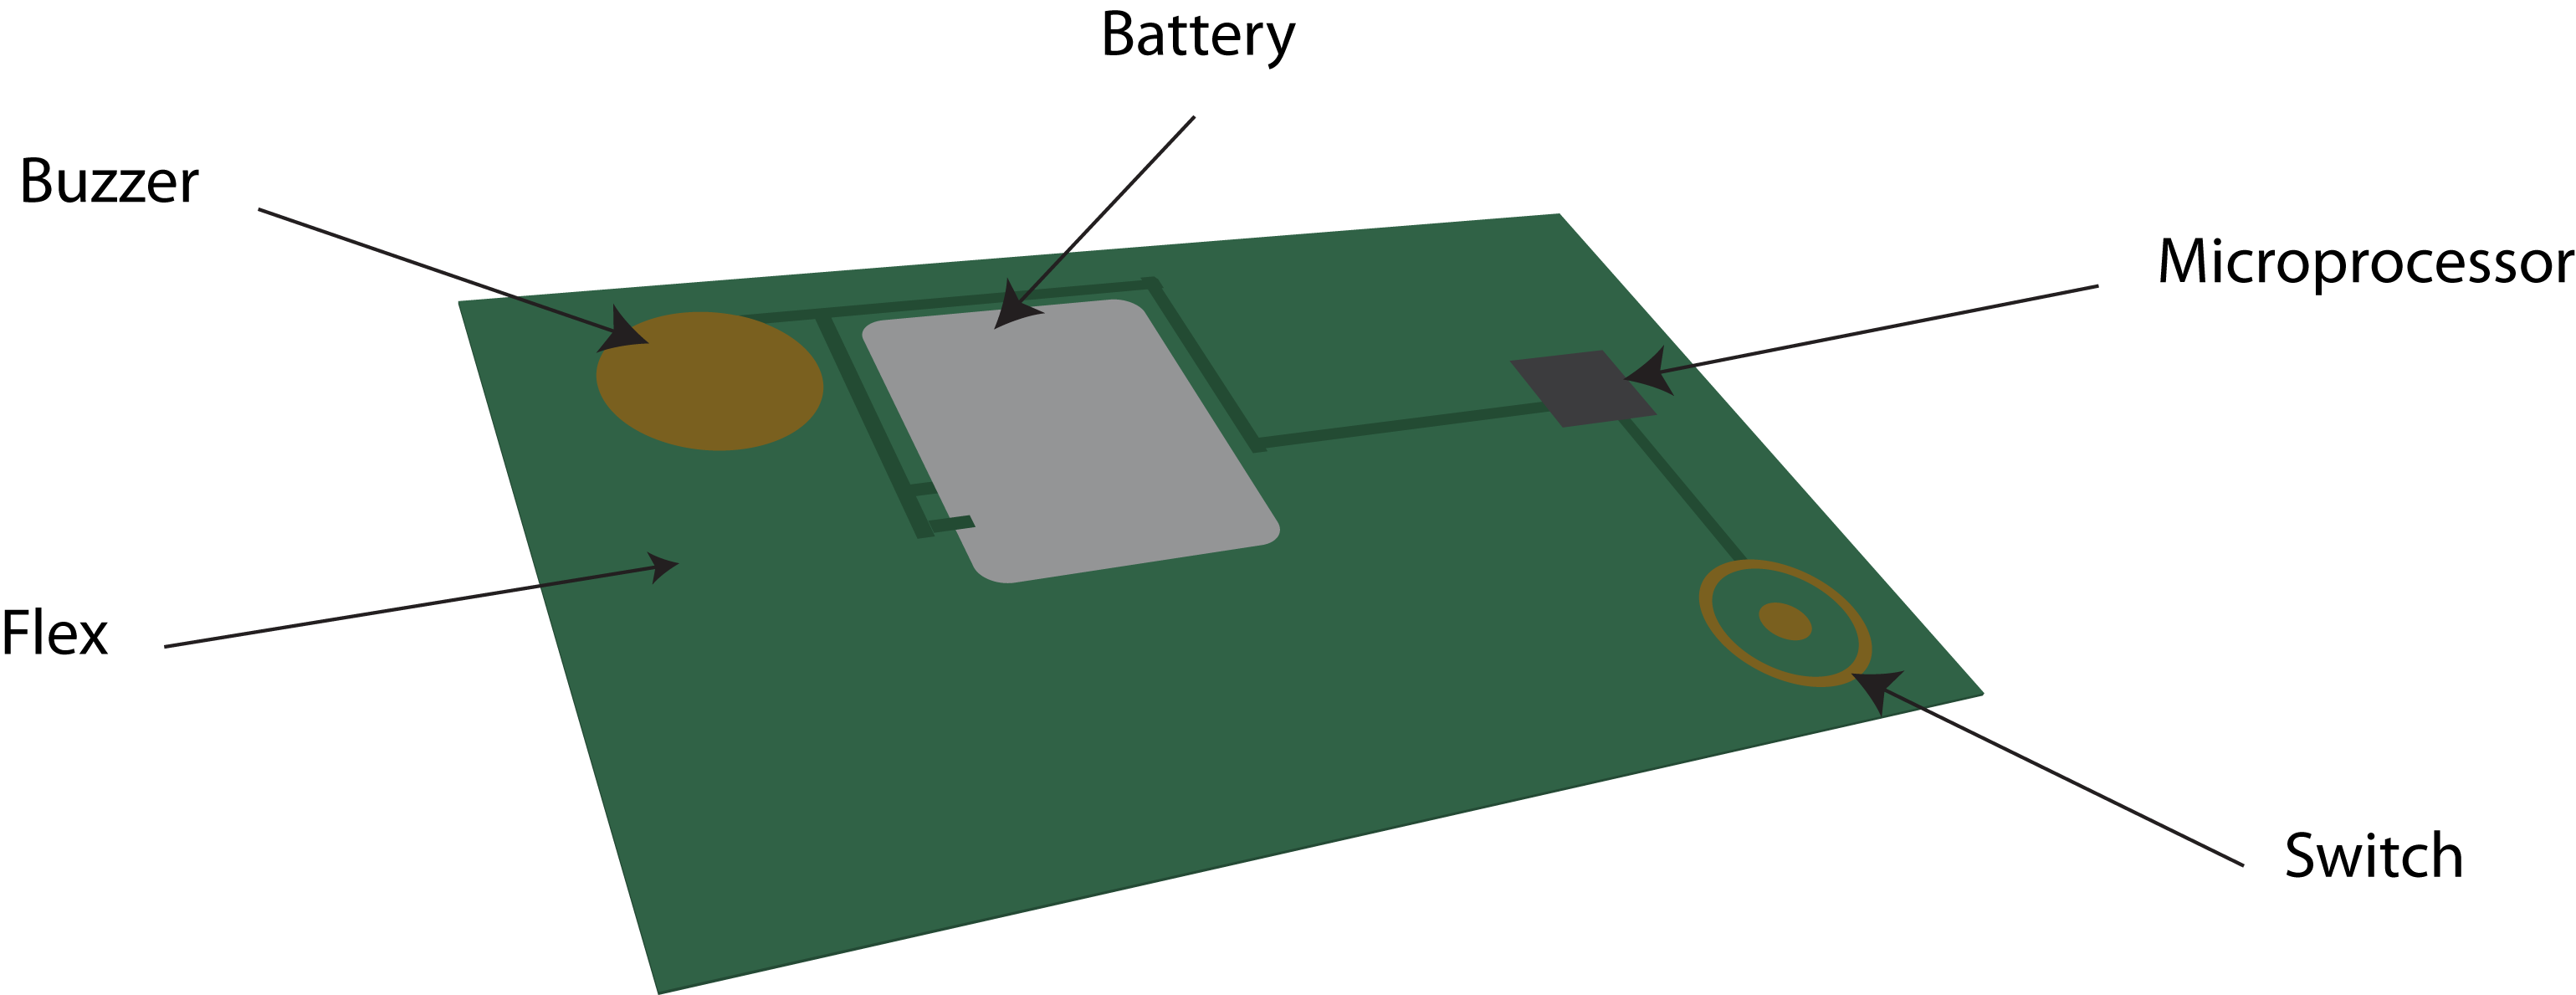
\includegraphics[scale=0.6]{images/carteinside}
  \caption{Schéma d’une carte acoustique}
  %\label{fig:auth}
\end{figure}

L’électronique embarquée est composée des éléments suivants :
\begin{itemize}
\item Un microcontrôleur
\item Une pile flexible de 3V – 10 mAh
\item Un buzzer
\item Un « bouton » qui déclenche la séquence acoustique.\\
\end{itemize}

Tous ces éléments ont été intégrés sur un circuit imprimé flexible, ou « flex ». L’ensemble des composants électroniques (microcontrôleur, buzzer et pile) sont directement soudés au « flex » par un processus de capillarité. Cet ensemble (Flex composants) est appelé Inlay et est intégré à l’intérieur de la carte PVC.

\subsection{Introduction à l’authentification forte}

Cette section a pour objectif de présenter le domaine de l’authentification forte, c'est-à-dire la problématique à laquelle il répond ainsi que les solutions qu’il propose.

\subsubsection{Définition de l’authentification}
S’authentifier, c’est prouver son identité (« je suis bien celui que je prétends être »).

\subsubsection{A quoi sert l’authentification}
Les nouvelles technologies de l’information et de la communication conduisent à une véritable explosion des échanges d’information sur les réseaux de télécommunication, tant dans l’univers professionnel que dans la vie quotidienne. Dans le même temps, les tentatives de fraude se multiplient, notamment par usurpation d’identité. L’authentification a pour objectif de renforcer la sécurité de ces échanges.
\newpage
\subsubsection{Les principaux moyens d’authentification}
L’utilisateur apporte la preuve de son identité en fournissant un élément:\\

\begin{itemize}
\item Que l’utilisateur est le seul à savoir (un mot de passe ou un secret par exemple);
\item Que l’utilisateur est le seul à détenir (un authentificateur: une carte, une clé, ...);
\item Qui caractérise l’utilisateur (empreinte digitale, image rétinienne, ...).\\
\end{itemize}

Chaque élément s’appelle « facteur d’authentification ». On parle d’authentification forte dès que le processus d’authentification fait appel à la combinaison d’au moins deux facteurs, par exemple un objet détenu par l’utilisateur et un mot de passe (code PIN) qu’il est le seul à connaître. Le processus d’authentification forte fait appel à un serveur d’authentification capable de comparer les éléments présentés par l’utilisateur avec les informations qu’il détient afin de délivrer – ou non – les droits d’accès.

\begin{figure}[!htbp]
  \centering
    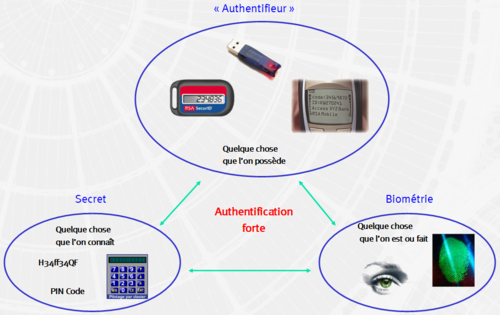
\includegraphics[scale=1]{images/relation}
  \caption{Représentation schématique de l’authentification forte}
  %\label{fig:auth}
\end{figure}

\subsubsection{Le mot de passe dynamique}
Il constitue une solution de plus en plus utilisée, notamment parce qu’il permet de conjuguer simplicité d’utilisation et robustesse en termes de sécurité. L’objet détenu par l’utilisateur (authentificateur ou « Token ») affiche, ou envoie directement, à intervalles réguliers ou à la demande, un mot de passe imprévisible et non réutilisable.\\

Au même instant, le serveur a calculé le même code pour cet utilisateur. Ceci est possible car l’authentificateur et le serveur disposent des mêmes éléments pour calculer le code. Il suffit alors au serveur de comparer le code calculé avec celui qui lui a été transmis. Le deuxième facteur associé à la solution, permettant de renforcer la sécurité en évitant le vol de l’authentificateur par un fraudeur lui donnant ainsi accès à l’information, est constitué d’un code personnel d’accès.

\subsubsection{Le marché de l’authentification}
Il connaît actuellement une très forte croissance, avec une prise de conscience de la nécessité de renforcer la sécurité de l’accès aux services en ligne et aux applications sensibles des entreprises. Dans le monde bancaire, le Federal Financial Institutions Examination Council (FDIC) a récemment publié un rapport incitant les banques à mettre en œuvre des solutions d’authentification forte à la mesure des risques encourus. Une étude récente de Froster Sullivan prévoit que le marché des authentificateurs, évalué à 248,1 millions de dollars en 2004, devrait bondir à 1,171 milliards de dollars en 2011.

\subsubsection{OATH}
OATH (Open AuTHentication) est une initiative d'un ensemble d'acteurs leaders du marché IT, travaillant ensemble afin de fournir une architecture de référence pour l'authentification forte. Basé sur des standards ouverts, OATH propose une interopérabilité entre les plateformes de validation (hardware et software) et tokens de fournisseurs différents afin d’offrir aux entreprises la possibilité de choisir et d’intégrer les meilleures offres du marché, afin de faciliter le déploiement et d'optimiser les coûts.

\subsection{Mécanismes de la séquence acoustique}
\subsubsection{Les constantes et variables essentielles}

L’algorithme permettant la génération de la trame acoustique est constitué de différentes fonctions cryptographiques qui vont calculer les cryptogrammes nécessaires à la génération du message. Il existe plusieurs valeurs importantes à traiter lors du calcul d’un cryptogramme. Ces valeurs sont de différentes natures, constantes ou variables, secrètes ou non, mais sont toutes enregistrées dans l’EEPROM lors de la personnalisation, c'est-à-dire lors de l’ultime étape de programmation du microcontrôleur. Ces différentes valeurs sont présentées dans le chapitre qui suit.\\

\textsl{Les clés cryptographiques (HOTP KeyA \& HOTP KeyB):}
Les clés cryptographiques sont des clés de quelques octets chacune. Ces clés sont générées par un logiciel développé par la société UINT. Ce logiciel fournit un couple de clés complètement aléatoires.

Ces deux clés sont des constantes et ne sont jamais modifiées par le programme sous peine de rendre le token inutilisable. Ces clés représentent un secret à protéger absolument car elles sont à la base du calcul du cryptogramme.\\

\textsl{Le compteur d’évènements (Event Counter):}
Le compteur d’évènements, comme son nom l’indique, comptabilise le nombre de pressions du bouton effectuées depuis la mise en route du token. Il est important de noter que ce compteur est chargé, lors de la personnalisation, avec une valeur aléatoire. Ce compteur représente le second secret à conserver car, tout comme les clés, il est utilisé dans le calcul du cryptogramme. Ce compteur a une taille de 8 octets.\\

\textsl{Le numéro de série (Id):}
Le numéro de série du token est codé sur 29 bits. Cette valeur permet de répertorier les tokens et de les associer avec leurs clés et leur compteur d’évènements. Le numéro de série n’est pas un secret, il est d’ailleurs transmis dans la trame acoustique. Maintenant que sont connues les quelques valeurs importantes utilisées lors de l’exécution du programme, il est possible de s’intéresser à la manière dont elles sont utilisées par l’algorithme de génération de la trame acoustique.


\subsection{Génération du cryptogramme acoustique}
Une fois les étapes préliminaires effectuées, il s’agit de calculer le cryptogramme à l’aide de fonctions spécifiques normalisées par des standards. Le chapitre qui suit explique la méthode adoptée afin de calculer ces données qui constituent le cœur du futur message à
émettre.

\subsubsection{La génération d’un HOTP}
Les informations qui suivent sont issues de la rfc4226, HOTP : An
HMAC-Based One Time Password Algorithm. Ce document
décrit un algorithme basé sur HMAC pour générer un mot de passe
unique (One Time Password). Ce document est le fruit d’un effort
conjoint des membres de la communauté OATH pour spécifier un
algorithme d’authentification qui est proposé librement à toute
organisation.

\subsubsection{La génération du cryptogramme}
Les différentes opérations nécessaires à la génération d’un HOTP définies, il s’agit maintenant de présenter l’utilisation qui est faite de ce HOTP. Afin de créer un cryptogramme qui va par la suite être encodé, le programme va générer deux HOTP, HOTPa et HOTPb, respectivement de 31 octets et 20 octets, à partir de deux clés distinctes, HOTP\_Keya et HOTP\_Keyb. Le programme va ensuite concaténer ces HOTP en leur ajoutant l’identifiant (Id) du token, et l’on obtient un cryptogramme représenté schématiquement ci-dessous :

\begin{figure}[!htbp]
  \centering
    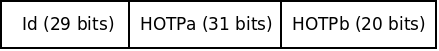
\includegraphics[scale=0.5]{images/otp}
  \caption{Représentation schématique du cryptogramme}
  %\label{fig:auth}
\end{figure}

Le cryptogramme est ainsi fabriqué. Cette étape constitue la dernière étape du processus de chiffrement des informations. Le cryptogramme peut maintenant être encodé afin de le rendre plus robuste au canal de transmission.

\subsubsection{L’encodage du cryptogramme}
L’encodage du cryptogramme est une étape qui consiste à mettre en forme et à ajouter de l’information au cryptogramme afin de le rendre plus robuste aux perturbations engendrées par le canal de transmission. L’encodage est composé de trois opérations distinctes :
\begin{itemize}
\item Le mélange du cryptogramme,
\item L’ajout d’un code de redondance cyclique au cryptogramme,
\item L’encodage convolutif du cryptogramme\\
\end{itemize}


\textbf{Le cryptogramme et les symboles}\\
Comme étudié précédemment le cryptogramme générer est constitué de 20 octets. Introduisons maintenant la notion de symbole. Un symbole est un quartet, mot de quatre bits. Le cryptogramme est donc constitué de 40 symboles. Chaque symbole appartient donc à l’ensemble de valeurs hexadécimales [0-F], et la représentation du message peut être la représentation hexadécimale. Ces symboles vont être transmis un à un par l’émetteur au destinataire afin que ce dernier puisse reconstituer le message dans son intégralité.\\

\textbf{Le mélangeur}\\
Comme vu précédemment, la séquence à encoder comporte un numéro de série fixe suivi de deux champs variables. Le but du mélangeur est d’éviter qu’une partie de la séquence soit stable d’une émission à l’autre, et donc que l’on retrouve les mêmes symboles aux mêmes emplacements dans la séquence. De plus si l’on imagine un canal de transmission qui détruit ou déforme systématiquement certain symboles, cet outil permet de disperser dans le temps les séquences difficilement décodables.\\

\textbf{L’ajout du CRC16 au message}\\
Les informations relatées dans ce paragraphe sont tirées d’un document intitulé A Painless Guide To CRC Error Detection Algorithms. Ce document explique en détail l’implémentation des différents Code de Redondance Cyclique (CRC).\\

Le but des techniques de détection d’erreurs est de permettre au destinataire d’un message transmis à travers un canal bruité de déterminer si le message a été corrompu. Pour ce faire, l’émetteur construit un code de contrôle, appelé somme de contrôle (checksum) par abus de langage, qui est fonction du message et le rajoute à la fin du message. A la réception, il suffit d’effectuer la même opération sur le message reçu, avec la même fonction et par comparaison des deux codes de contrôle on peut tester la validité du message. L’exemple qui suit est une illustration du fonctionnement d’un code de contrôle très simple. Il s’agit en fait d’additionner la valeur de chaque octet.

\begin{center}
\begin{tabular}{|l|l|}
\hline
Message & 6 23 4\\ \hline
Message avec code de contrôle & 6 23 4 33\\ \hline
Message reçu & 6 2{\color{red}7} 4 33\\ \hline
\end{tabular}
\end{center}

A la réception on s’aperçoit aisément qu’il y une erreur de transmission. Dès lors on peut redemander l’envoi des données ou bien ignorer le message en fonction de l’application. L’exemple présenté ci-dessus n’est pas utilisé en télécommunication, domaine dans lequel on lui préfère des codes de contrôle plus complexes permettant de détecter des erreurs mais aussi d’en corriger certaines.\\

L’idée de base des algorithmes CRC est de traiter le message comme un grand nombre binaire, de le diviser par un second nombre binaire constant (le polynôme), et de considérer le reste de la division comme le code de contrôle à ajouter à la fin du message. Les différents algorithmes diffèrent par la valeur du polynôme utilisé, la taille du code de contrôle calculé et la valeur initiale du registre de calcul.\\

\textbf{Le codage convolutif}\\
En plus du calcul et de l’ajout du CRC à la séquence, un codage convolutif est appliqué à cette séquence afin de la renforcer et de compléter le code de contrôle.\\

Un codeur suivant une loi de codage convolutif associe N bits « codés » à K bits d'information. Chaque bloc de N éléments binaires transmis dépend non seulement du bloc de K éléments présents à son entrée mais aussi des m blocs précédents. Le codeur est constitué de m registres à décalage de K éléments binaires. Une logique combinatoire constituée de N générateurs linéaires de fonctions algébriques génère les blocs de N éléments binaires fournis par le codeur.



\subsubsection{La modulation acoustique}
La modulation acoustique des symboles est l’ultime étape de la chaîne de traitement du signal. Elle consiste à traduire un symbole par un son au travers d’un buzzer. Cette opération permet d’adapter le message électronique au canal de transmission utilisé qui est celui de la voix téléphonique. Il a donc fallu prendre en considération la bande passante de ce canal qui est [300 Hz; 3400 Hz]. Les sonorités produites par le buzzer devront donc être des fréquences comprises dans cette bande passante.\\

\textbf{Principe}\\
Lorsque l’on excite le buzzer avec un signal, le buzzer oscille à la fréquence propre du signal et émet un son à cette fréquence. Donc pour résumer, si on arrive à générer un signal sinusoïdal pur à partir du microcontrôleur l’on peut représenter aisément un symbole par une fréquence et donc une sonorité. Malheureusement il est plutôt complexe de réaliser cette opération et l’on préfère générer un signal créneau (état bas = 0, état haut = 1) dont la fréquence est celle du symbole à émettre. En effet un signal carré peut être considéré comme une somme de sinusoïdes, dont la principale, appelée aussi fondamentale, oscille à la fréquence du signal. Enfin en choisissant judicieusement les fréquences pour chaque symbole on s’affranchit de tout risque de « débordement » d’une harmonique sur la plage d’un autre symbole.
Une fois les sonorités émises, c’est au microphone du téléphone ou de l’ordinateur de transcrire les vibrations acoustiques au système de traitement qui les numérise et les transmet au destinataire.

\subsubsection{Organigramme de fonctionnement de la carte acoustique}
L’organigramme ci-après présente les différentes étapes de l’algorithme de la carte acoustique. Les variables y sont représentées en jaune, les constantes secrètes en rouge, les algorithmes en bleu et la restitution des données en vert. Les flèches indiquent le sens de déroulement de l’algorithme général.

\begin{figure}[!htbp]
  \centering
    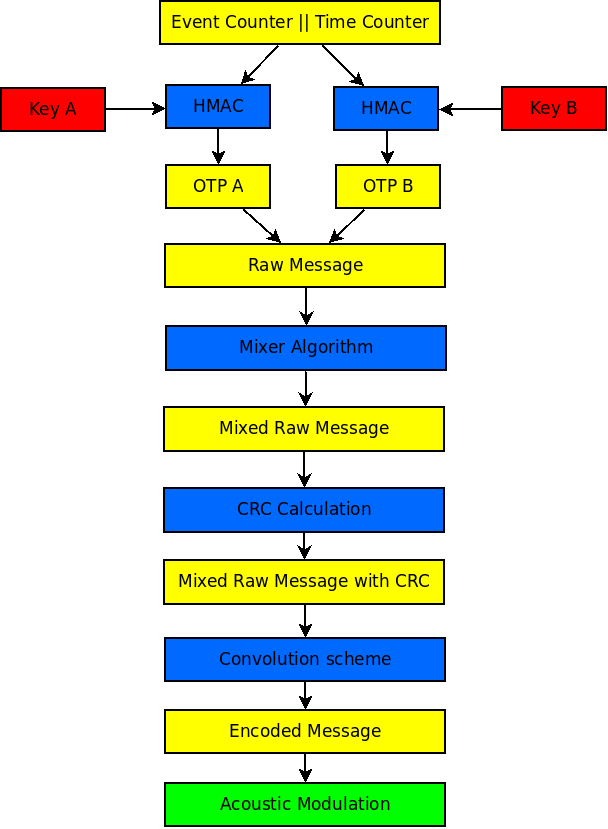
\includegraphics[scale=0.6]{images/organigramme}
  \caption{Fonctionnement de la carte acoustique}
  %\label{fig:auth}
\end{figure}





